\documentclass[12pt]{article}
\usepackage{graphicx}
\usepackage{amsmath}
\usepackage{mathtools}
\usepackage{gensymb}

\newcommand{\mydet}[1]{\ensuremath{\begin{vmatrix}#1\end{vmatrix}}}
\providecommand{\brak}[1]{\ensuremath{\left(#1\right)}}
\providecommand{\norm}[1]{\left\lVert#1\right\rVert}
\newcommand{\solution}{\noindent \textbf{Solution: }}
\newcommand{\myvec}[1]{\ensuremath{\begin{pmatrix}#1\end{pmatrix}}}
\let\vec\mathbf

\begin{document}
\begin{center}
\textbf\large{CLASS-9\\CHAPTER-10 \\ CIRCLES}

\end{center}
\section*{Excercise 10.5}

Q1. In Figure 1. $\vec{A,B,C}$ are the three points with centre $\vec{O}$ such that $\angle$BOC=30\degree and $\angle$AOB=60\degree. If $\vec{D}$ is a point on the circle other than the arc ABC, find $\angle$ADC
\section*{\large Solution}
\begin{figure}[h!]
\centering
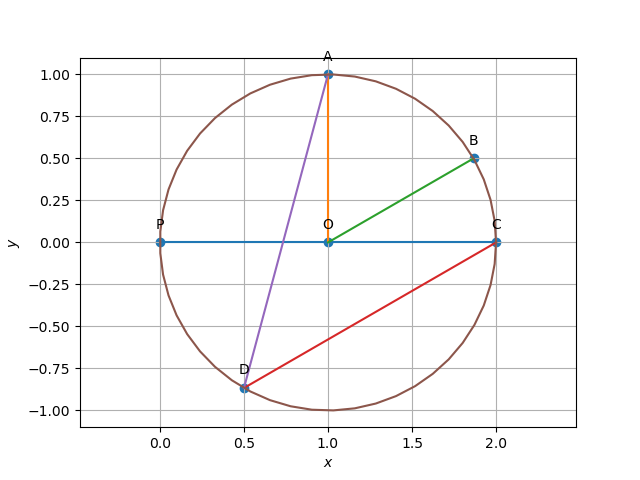
\includegraphics[width=\columnwidth]{figs/circle2.png}
\caption{}
\end{figure}
\section*{\large Construction}


\begin{table}[htbp]
 \begin{center}
    \begin{tabular}{|l|c|c|c|c|c|c} \hline \textbf{Symbol}
  & \textbf{value} & \textbf{Description} \\
 \hline
	    r &1 unit& Radius of OA and OB\\ \hline
	    $\vec{O}$ &\myvec{0\\r} & Centre of the circle\\ \hline
	    $\vec{C}$ &\myvec{1\\0} & Standard basis vector $\vec{e}_1$\\ \hline
	    $\alpha$ & 30\degree&Angle between vectors $\vec{B} \text{ and } \vec{C}$ w.r.t $\vec{O}$ \\ \hline
	    $\beta$ & 60\degree&Angle between vectors $\vec{A} \text{ and } \vec{B}$ w.r.t $\vec{O}$ \\ \hline
	    $\gamma$ & ??&Angle between vectors $\vec{A} \text{ and } \vec{C}$ w.r.t $\vec{D}$ \\ \hline
\end{tabular}   
\end{center}
\caption{\label{table:dummytable} }
\end{table}

\section*{\large Assumptions}
\begin{enumerate}
	\item Let $\vec{P}$ be a point on the circle such that by expandig OC upto $\vec{P}$ we get diameter POC.
\item To find $\angle$ADC let the circle be unit circle and diameter POC on x axis.
\item Take three points $\vec{C,A,D}$ and $\alpha$,$\beta$,$\gamma$ be three angles made by the points $\vec{C,A,D}$ with respect to diameter POC.
\end{enumerate}
From the Figure 1:
\begin{align}
\alpha = {\angle POC}= 180\degree, 
\beta= {\angle POA} = 90\degree,
\gamma = {\angle POD}=300\degree
\end{align}
\section*{Verification:}
From assumptions the vector points $\vec{C,A,D}$ be
\begin{align}
	\vec{C} = \myvec{\cos\alpha\\\sin\alpha},
	\vec{A} = \myvec{\cos\beta\\\sin\beta},
	\vec{D} = \myvec{\cos\gamma\\\sin\gamma}
\end{align}
Let AC be the chord that subtends angles at the center $\vec{O}$ and at point $\vec{D}$. The cosine of the angle subtended at point $\vec{D}$ is given by
\begin{align}
	\cos(\angle ADC) = \frac{\vec{(A-D)^\top(C-D)}}{\norm{\vec{A-D}}\norm{\vec{C-D}}}
	\label{eq:3}
\end{align}
Where
 \begin{align}
	 \vec{A-D}& = \myvec{\cos\beta - \cos\gamma\\\sin\beta - \sin\gamma},
	 \vec{C-D} = \myvec{\cos\alpha - \cos\gamma\\\sin\alpha - \sin\gamma}\\
	 \label{eq:5} \vec{(A-D)^\top(C-D)}&= 4\sin\frac{\alpha-\gamma}2\sin\frac{\beta-\gamma}2\cos\frac{\alpha-\beta}2\\
	 \norm{\vec{A-D}}\norm{\vec{C-D}}& = 4 \sin\frac{\alpha-\gamma}2\sin\frac{\beta-\gamma}2
	\label{eq:6}
\end{align}
Substituting \eqref{eq:5} and \eqref{eq:6} in \eqref{eq:3},
\begin{align}
	\cos(\angle ADC) &= \frac{4\sin\frac{\alpha-\gamma}{2}\sin\frac{\beta-\gamma}{2}\cos\frac{\alpha-\beta}{2}}{4 \sin\frac{\alpha-\gamma}2\sin\frac{\beta-\gamma}2}\\
	\cos(\angle ADC) &= \cos\frac{\alpha-\beta}{2}
	\label{eq:11}
\end{align}
By substituting $\alpha$ and $\beta$ values in \eqref{eq:11}
\begin{align}
\angle ADC = \frac{\alpha-\beta}{2}=\frac{(180\degree - 90\degree )}{2}=45\degree
\end{align}



\end{document}
